\documentclass[12pt]{article}
\usepackage[margin=1in]{geometry}
\usepackage{timeline}
\usepackage{graphicx}
\usepackage{color}
\usepackage{float}
\usepackage{hyperref}
\usepackage{mathtools}

\usepackage[style=authoryear, backend=bibtex]{biblatex}
\addbibresource{final_bib.bib}
\nocite{*} 

\usepackage{listings}
\lstset{ %
language=Java,                % choose the language of the code
basicstyle=\footnotesize,       % the size of the fonts that are used for the code
numbers=left,                   % where to put the line-numbers
numberstyle=\footnotesize,      % the size of the fonts that are used for the line-numbers
stepnumber=1,                   % the step between two line-numbers. If it is 1 each line will be numbered
numbersep=5pt,                  % how far the line-numbers are from the code
backgroundcolor=\color{white},  % choose the background color. You must add \usepackage{color}
showspaces=false,               % show spaces adding particular underscores
showstringspaces=false,         % underline spaces within strings
showtabs=false,                 % show tabs within strings adding particular underscores
frame=single,           % adds a frame around the code
tabsize=2,          % sets default tabsize to 2 spaces
captionpos=b,           % sets the caption-position to bottom
breaklines=true,        % sets automatic line breaking
breakatwhitespace=false,    % sets if automatic breaks should only happen at whitespace
escapeinside={\%*}{*)}          % if you want to add a comment within your code
}

\author{Advisor/Client: Dave Hale \\ Team Members: Colton Kohnke}
\title{GPGN438 Senior Design: \\ Exploratory Seismic Data Analysis in the Field}
\date{April 28th, 2014}

\begin{document}
\maketitle
\newpage

\section{Executive Summary}

Seismic surveys take a significant amount of time and money to complete correctly. This project's purpose is to develop software for the Colorado School of Mines (CSM) to aid with viewing seismic survey data and survey geometry in the field. The software is also able to help catch errors in the field. Finally, it can serve as a teaching tool for the students of the Colorado School of Mines Geophysics Field Camp to help them better comprehend seismic surveys. \\

The software accomplishes this by reading the SEGD files from the Sercel recording truck along with the station locations from a GPS unit. This data is then plotted in map and section view in order to give snapshots of the seismic survey. The survey can then be explored in map view as stations and the shot records can be displayed based off of user input. This exploration comes in the form of dynamic display of shot records, stacks of shot records, and common channel sections.\\

Basic processing can then be completed in a dynamic and interactive way. The current processes that are included are gain, lowpass filtering, and time-power amplitude-gain. The program handles the display of the processed data from user controlled sliders. The plot of the selected data is updated in real-time as the user moves the slider. This allows the user to explore multiple different configurations of gain, lowpass filtering, and time amplitude gain in a short amount of time. This allows the user to find the best parameters for viewing the data.\\

The software is ready for use in the 2014 Geophysics Field Camp. The software has been developed to be quick and accurate in a field setting to look at the collected seismic data. It has also been developed to be easy for the end user to utilize. While the current version of the software is useful, there are many features missing from the software that would make this program essential to the Geophysics Field Camp. 

\newpage
\tableofcontents
\listoffigures
\listoftables
\newpage

\section{Problem Statement}

This project is to develop software in Java that lets the user explore the seismic survey while in the field. The survey exploration includes the interactive display of survey geometry and seismograms. This software will also be able to perform simple processing tasks in the field. This is a new tool to be used at the Geophysics Field Camp with the intention to give a graphical user-interface (GUI) to the display of the seismic survey geometry. This software will also be used as a teaching tool for the students to give them a better understanding of the seismic survey and data.

\section{Introduction \& Background}

Seismic data collection is an expensive operation in both time and money. In the field, it is in the data collector's best interest to guarantee high quality data is obtained. Poor data quality is a waste of time and money in the field, and this hinders processing when back in the office. \\

ProMAX is the current system used in the field to view the seismic data coming in from the recording truck. This system, while good for extensive processing, is not quick enough to display survey data in an interactive way. There is a need for a new tool that can be easily deployed in the field and has the ability to quickly display survey geometry, associated shot records, and other information dynamically based off of user input.

\section{Deliverables to Client}

The deliverables of this project include two main items. The first is a program written in Java that accomplishes the design objectives outlined in the next section. The second deliverable will be a documentation of the code using standard Java practices and a compilation of the documentation using the Javadoc tools provided by Sun Microsystems. This documentation will take the appearance of standard Java web-based documentation, much like the documentation found in the Mines Java Toolkit. The software will also come with commented code in order to aid further development. 

\section{Design Objectives}
\subsection{Interactive Display of Survey Geometry}

The first objective is to be able to import station (flag) locations. This needs to be accomplished from a variety of GPS sources including CSV, Garmin GPX, and tab-delimited text files. The GPS coordinates need to then be converted to UTM for display. Once the conversion is applied, the next step is to plot the locations in map view. The user then needs the ability to import and read elevations from the USGS Digital Elevation Maps. Once the elevations are read, the software plots an elevation profile of the survey. Finally, the user needs to have the option of exporting all the GPS data for use in other situations (e.g. aiding the gravity survey). The columns that are exported are listed in Table \ref{TAB:GPS}.

\begin{table}[h]
\caption{GPS Export Spreadsheet Fields}
\centering
\begin{tabular}{ c | c | c | c}
  \hline                  
  StationID & UTM Easting & UTM Northing & Elevation \\
  \hline
\end{tabular}
\label{TAB:GPS}
\end{table}

The second objective is to be able to compute source and receiver locations. This is done for each valid shot FFID (Field File ID) by using the Sercel SEGD files to determine the source station number, live recording channels, and receiver station numbers. This data is then plotted in map view on top of the plot of GPS points. Some FFIDs correspond to bad shots and these are ignored by the program routines.  \\

Finally, there is a slider to select and show points corresponding to each FFID that will provide a graphical history of the seismic survey and help to catch errors. 

\subsection{Interactive Display of Seismograms} 

The first step to displaying the seismograms is to convert the Sercel SEGD files (bytes) to an array of an array of floats (2D float array). Once this is accomplished, the seismograms are interactively displayed by using the mouse in the plot of GPS locations. As the user moves the mouse along the seismic survey in map view, a plot of the shot record updates in real time. Another method to display the seismograms is to combine the shots within a circle that the user draws in map view. Finally, the user is able to define a specific channel, and all loaded shots within that channel will be displayed. This common-channel gather is controlled by a slider, and updates in real time as the user changes the channel number to display. \\

\subsection{Interactive Gain, Amplitude Balancing and Lowpass Controls}

All of the displays are useless unless the data can be seen. Therefore, interactive controls for gain, amplitude balancing, and lowpass filtering (Butterworth) have been implemented. This was accomplished by using sliders embedded in the graphical user-interface. As the user moves the slider, the plot of selected shot records updates in real time.

\subsection{Other Requirements}

Speed is a top priority when working in the field. Decisions are typically made quickly in order to move the survey along at a reasonable rate. If this software is fast enough, it can be used as a supplement to those decisions. The field camp data set is small enough that speed should not be an issue. If the data set was larger, more issues would arise because currently all of the data from the survey is stored in the memory Java allocates from RAM.\\

The graphical user-interface must be easy to use. The layout of the controls must be logical and follow a sequential order.  If there are errors thrown in the process of importing and plotting the data, the user needs to be made aware of what steps they are missing. This will accelerate the learning curve for this new tool and make it easier to use in the field.

\section{Decision-making \& Assessment of Alternative Approaches}

The decisions during the main software development section of this project deal with efficiency. Choices in the field need to be made quickly and as a result, the software needs to be able to perform operations efficiently to keep pace. If the software is called to display a seismic shot, it needs to be able to find the data and display it in the least amount of operations. Similarly, if an operation is applied to a set of data, it should be applied in the least amount of compute time. \\

The software is not currently optimized for speed because that would slow down development. However, specific places in the software have been marked for efficiency improvements during the testing phase. One area that has been marked for optimization is the storage of the data from the SEGD files. Currently, shots are stored as an ArrayList which is traversed linearly. In Big-O Notation, this causes an O($n^2$) search time where $n$ is the length of the List. A much faster implementation would be a Binary Search Tree which has O($n$) traversal time. Another option is implementing a Hash Table which returns a value in near constant time, O($1$). \\

The decisions during the final stages of the project revolve around end user usability. These choices include aesthetic placement of tools in the software to create a logical progression of tasks for the end user. The decisions in this phase will also revolve around how to lay out the documentation for the end user.

\section{Design Solution}

The tool that is being used in this design project is simulation. Each method that is written is tested by calling a main method that tests the code with the 2013 Field Camp seismic data. These simulations provide the developer with real data to test the software. It also provides data about speed and efficiency to make sure the software is meeting the required benchmarks. \\

In addition, before a feature is integrated into the larger code, it is tested for errors and correct implementation. This speeds up the development process because it limits the area where bugs can occur at a time. When the bugs occur, they are fixed in the responsible code and retested for consistency. \\ 

The software also utilizes modular design. This is a technique that separates the main program into several different smaller programs that contain everything they need to achieve their own functionality. The main program knows about, and controls, all the modules, but the modules do not know about each other. This aids future development because new modules are easy to add without changing much of the main program.

\section{Implementation Plan}
\subsection{Safety}

The main safety concern of this project is the ergonomics of the developer. This project does not require field work or manual labor in the traditional sense. However, it does require a significant amount of time to be spent coding at a computer which may cause irritation of the wrist or forearm. The developer will mitigate the risk of encountering this problem by taking breaks, stretching, and using correct posture while at the workstation.

\subsection{Timeline}

\begin{figure}[H]

\begin{timeline}{2013}{2015}{200}{300}
  \categorylabel{Senior Design Timeline}{60}
  
  \MonthAndYearEvent{9}{2013}{Project start}
  \MonthAndYearEvent{10}{2013}{Java base using Mines JTK Demo files.}
  \MonthAndYearEvent{11}{2013}{Sercel SEGD reading and plotting Jython code converted to Java.}
  \MonthAndYearEvent{11}{2013}{Demo with interactive plots created}
  \MonthAndYearEvent{1}{2014}{Core features implemented}
  \MonthAndYearEvent{1}{2014}{Alpha testing starts}
  \MonthAndYearEvent{1}{2014}{Code optimization begins}
  \MonthAndYearEvent{3}{2014}{Beta testing begins}
  \MonthAndYearEvent{3}{2014}{Documentation writing begins}
  \MonthAndYearEvent{5}{2014}{Final product ready for use at CSM Field Camp 2014}
  
\end{timeline}
\caption{Senior Design Project Timeline}
\end{figure}

\subsection{Budget 1: Actual}

No budget is required for the actual project, as the project does not require any traveling or other expenditures outside the realm of a standard class at CSM.

\subsection{Budget 2: Professional}

Ideally to get a working product to the client, the following budget in Table \ref{TAB:BUG} would be used in a professional setting. 

\begin{table}[h]
\caption{The Professional Budget}
\begin{tabular}{ l | l | l || l | l}
  \hline                        
  Item & Base Cost & Quantity & Total & Notes \\ \hline
  Developers & \$20.00/hr & 360 & \$7,200 & 2 Devs for 4 work weeks.\\
  Continued Support & \$15.00/hr & 260 & \$3,900 & 1 Dev at 5 hours/week for 1 year.\\ \hline
  Base Total & & & \$11,100 & \\
  Overshoot & & & \$1,110 & 10\% addition\\ \hline
  Total & & & \$12,210 & \\
  \hline  
\end{tabular} 
\label{TAB:BUG}
\end{table}

In reality, a project of this magnitude would likely cost much more than anticipated above. The main cost is dependent on the size of the team developing the program, their skill level, and what features are being implemented. These extra variables make discerning an actual budget more complicated. This project could potentially be funded by selling the program to clients. To market this program, more hurdles would have to be overcome and an expanded budget would be created.

\section{Program Design}

The program is divided into several levels of command to simplify the program and aid further development. The highest level, the PlotTest class, initiates the program by constructing the three plot classes, BasePlot, ResponsePlot, and ElevPlot. The BasePlot class handles the map view data that is plotting on the Base Plot (see Section \ref{SUBSEC:BPC}). The ResponsePlot class handles the seismic shot data on the Response Plot (see Section \ref{SUBSEC:RP}). Finally, the ElevPlot handles the plotting of the survey elevation data (see Section \ref{SUBSEC:EP}). The three classes act as secondary controllers to the program. Finally, there are multiple helper classes that aid the three plots in calculating and obtaining data from multiple sources. \\

From the viewpoint of modular programming, the SeisPlot class is the main program. The three plot classes consist of a single module because they are able to talk to each other and back to the main SeisPlot class. Finally, the helper classes can be combined into specific modules that are called by the SeisPlot class. The main SeisPlot class can call methods in the plot classes and the plots call methods from the helper classes. The data returned then goes back into the SeisPlot class so the next action can happen.

\subsection{Main Controller - SeisPlot Class}

The Main Controller of the program is the SeisPlot Class. Inside the SeisPlot class there are three internal classes (BasePlot, ResponsePlot and ElevPlot) for the three different plots. The SeisPlot class is responsible for storing data that is imported, creating menu items, and for handling different modes for the plots. The SeisPlot class is also responsible for taking information passed to it by its internal classes and then handling the parameters of what needs to be updated next. \\

\subsubsection{Menu Items}

The first Menu is the "File" Menu. Under this header, there are two options. The first option is "Save as PNG"  which will bring up a file browser (Figure \ref{FIG:PNG}) that will save the current plot to a PNG image file. The plot that is saved will be the plot from the window that the menu item is selected from.

\begin{figure}[h]
\centering
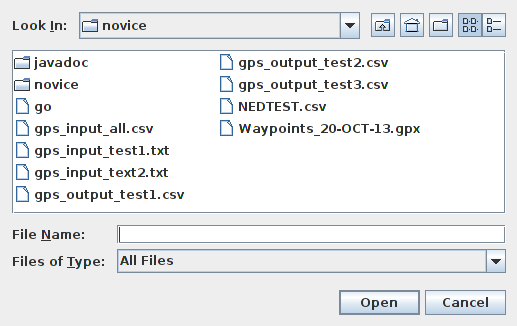
\includegraphics[width=0.75\textwidth]{./figs/fig0.png}
\caption{JFileChooser for importing data.}
\label{FIG:PNG}
\end{figure}

The second option under the "File" menu is "Exit," which will close the program and release all allocated memory. \\

The second Menu is the "Mode" menu. This menu allows for switching between the various modes that are available. At the time of this writing, the modes that exist are "Zoom Mode," "Roam Mode," "Circle Mode," and "Channel Mode." Each Mode has a different function for the various plots, and their role will be discussed in those sections. The Modes also have icons on the right side of the base map. \\

The "Tools" Menu contains methods to import and manipulate data. The "Get HandHeld GPS" option will import GPS points from a Tab Separated Value (TSV, extension ".txt"), Comma Separated Value (CSV, extension ".csv") or Garmin GPX file (extension ".gpx"). The file type is automatically detected based on the file extension. This method assumes that the TSV and CSV data is of a format similar to Table \ref{TAB:GPS2}. Currently, any elevation values are ignored in favor of reading the Nation Elevation Database (NED) files. Also, the data must be in decimal latitude and longitude and will be converted to UTM Easting and Northing upon import. Importing GPS data will update the Base Map plot with the GPS points (see Section \ref{SUBSEC:BPC}).\\

\begin{table}[h]
\caption{GPS Import Spreadsheet}
\centering
\begin{tabular}{ c | c | c}
  \hline                  
  Station ID & Latitude (decimal) & Longitude (decimal) \\
  \hline
\end{tabular}
\label{TAB:GPS2}
\end{table}

The next item is "Import NED Files" and it adds the NED GridFloat files to the SeisPlot's list of NED files to search through. In the 2012 Pagosa Spring Colorado Field Camp, the seismic survey was located on the edge of two NED files, so the program was written to be able to handle multiple NED files. This method requires the GridFloat file (extension ".flt") to be in the same directory as the Header file (extension ".hdr"). "Read Elevations from NED" will take the current imported GPS points and the imported NED Files and update the GPS point elevation fields. This happens based on the GPS point's latitude and longitude. The Elevation Plot is then updated with the profile of the survey (see Section \ref{SUBSEC:EP}). \\

"Export GPS to CSV" will export the GPS data to a CSV file. The format of the export is defined in Table \ref{TAB:GPS}. Exporting the data will not erase the data stored in memory. \\

"Import SEGD Directory" will open up a file browser and when the user selects a directory, all of the Segd files (extension ".segd") of Sercel's format will be read and imported into memory. "Import SEGD File(s)" does the same thing, but the user must specify a specific SEGD file, or group of files, to import. \\

The "Test" Menu item contains methods that the developer was testing before integrating into a different Menu. The current test items are "Clear Data" and "Plot Controls." The first item, "Clear Data," is for making testing easier and it clears the storage for SEGD, GPS data and NED files. Finally, "Plot Controls" displays sliders that are used for controlling the gain, lowpass filtering and the amplitude balancing. More information on the "Plot Controls" item is discussed in the ResponsePlot section below (see Section \ref{SUBSEC:RP}).

\subsection{Secondary Controller - BasePlot Class}
\label{SUBSEC:BPC}

The main purpose of the BasePlot class is to display the survey in map view. The other purpose of this plot is to allow for exploration of the seismic survey geometry in a dynamic environment. \\

\begin{figure}[h]
\centering
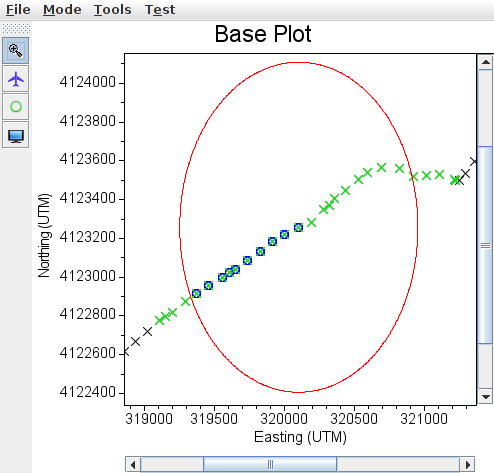
\includegraphics[width=0.75\textwidth]{./figs/fig1.png}
\caption{The base map after GPS and SEGD data has been imported during Roam Mode with summation turned on. This plot shows selected shots (the blue circles inside the red circle), the active receiver locations (green crosses) and the station locations (black crosses).}
\label{FIG:BP}
\end{figure}

In Figure \ref{FIG:BP} we see the map view of the GPS in Roam Mode and a distance of summation defined. The legend for this plot is independent of mode and defined as follows. The black cross icons define where the GPS points are located. The blue circles define which shots are currently selected. The green crosses define the receivers that are currently active. The red circle defines the spatial limits of shots that are currently selected.

\subsubsection{Zoom Mode}

In Zoom Mode, the base map may be zoomed in and explored using the scroll bars. This allows for a specific part of the seismic survey to be highlighted. To zoom, click and drag a box of interest and then let go of the mouse to zoom. To zoom out to the full view, right click the mouse. 

\subsubsection{Roam Mode}

When Roam Mode is selected, the user can click and drag their mouse along the seismic line in order to dynamically select shots. The shot record that is selected is dependent on the user's current mouse location. The program will determine the closest GPS station to the mouse and then select the nearest shot to that GPS location. As the user moves their mouse, the Base Plot updates with the new selected shot location. At any time, the user may change the Summation Range Slider to select more (or less) shot records to select. This selection is based from the last closest GPS point to the mouse, meaning in locations with no data, no shot points will be selected.

\subsubsection{Circle Mode}

Circle Mode behaves much like Roam Mode, but instead of clicking and dragging the mouse to display the nearest shot, the user clicks and drags to define a circular range. As the user moves their mouse to define a range, the Base Map will update by selecting the shots within that range. The first point the user defines is the center of the circle and from there they drag the mouse to define the radius. In most cases, the circle will actually be elliptical due to the scale of the axes of the Base Plot.

\subsection{Secondary Controller - ResponsePlot Class}
\label{SUBSEC:RP}

The ResponsePlot Class is responsible for plotting the seismic data. Depending on the mode, different types of plots are created.  In the case of Roam Mode and Circle Mode, a stack of selected shots is displayed. In the case of Channel Mode, a common channel section is created. Figure \ref{FIG:RP} shows a standard display in Roam Mode with no summation or in Circle Mode with only one selected shot.

\begin{figure}[h]
\centering
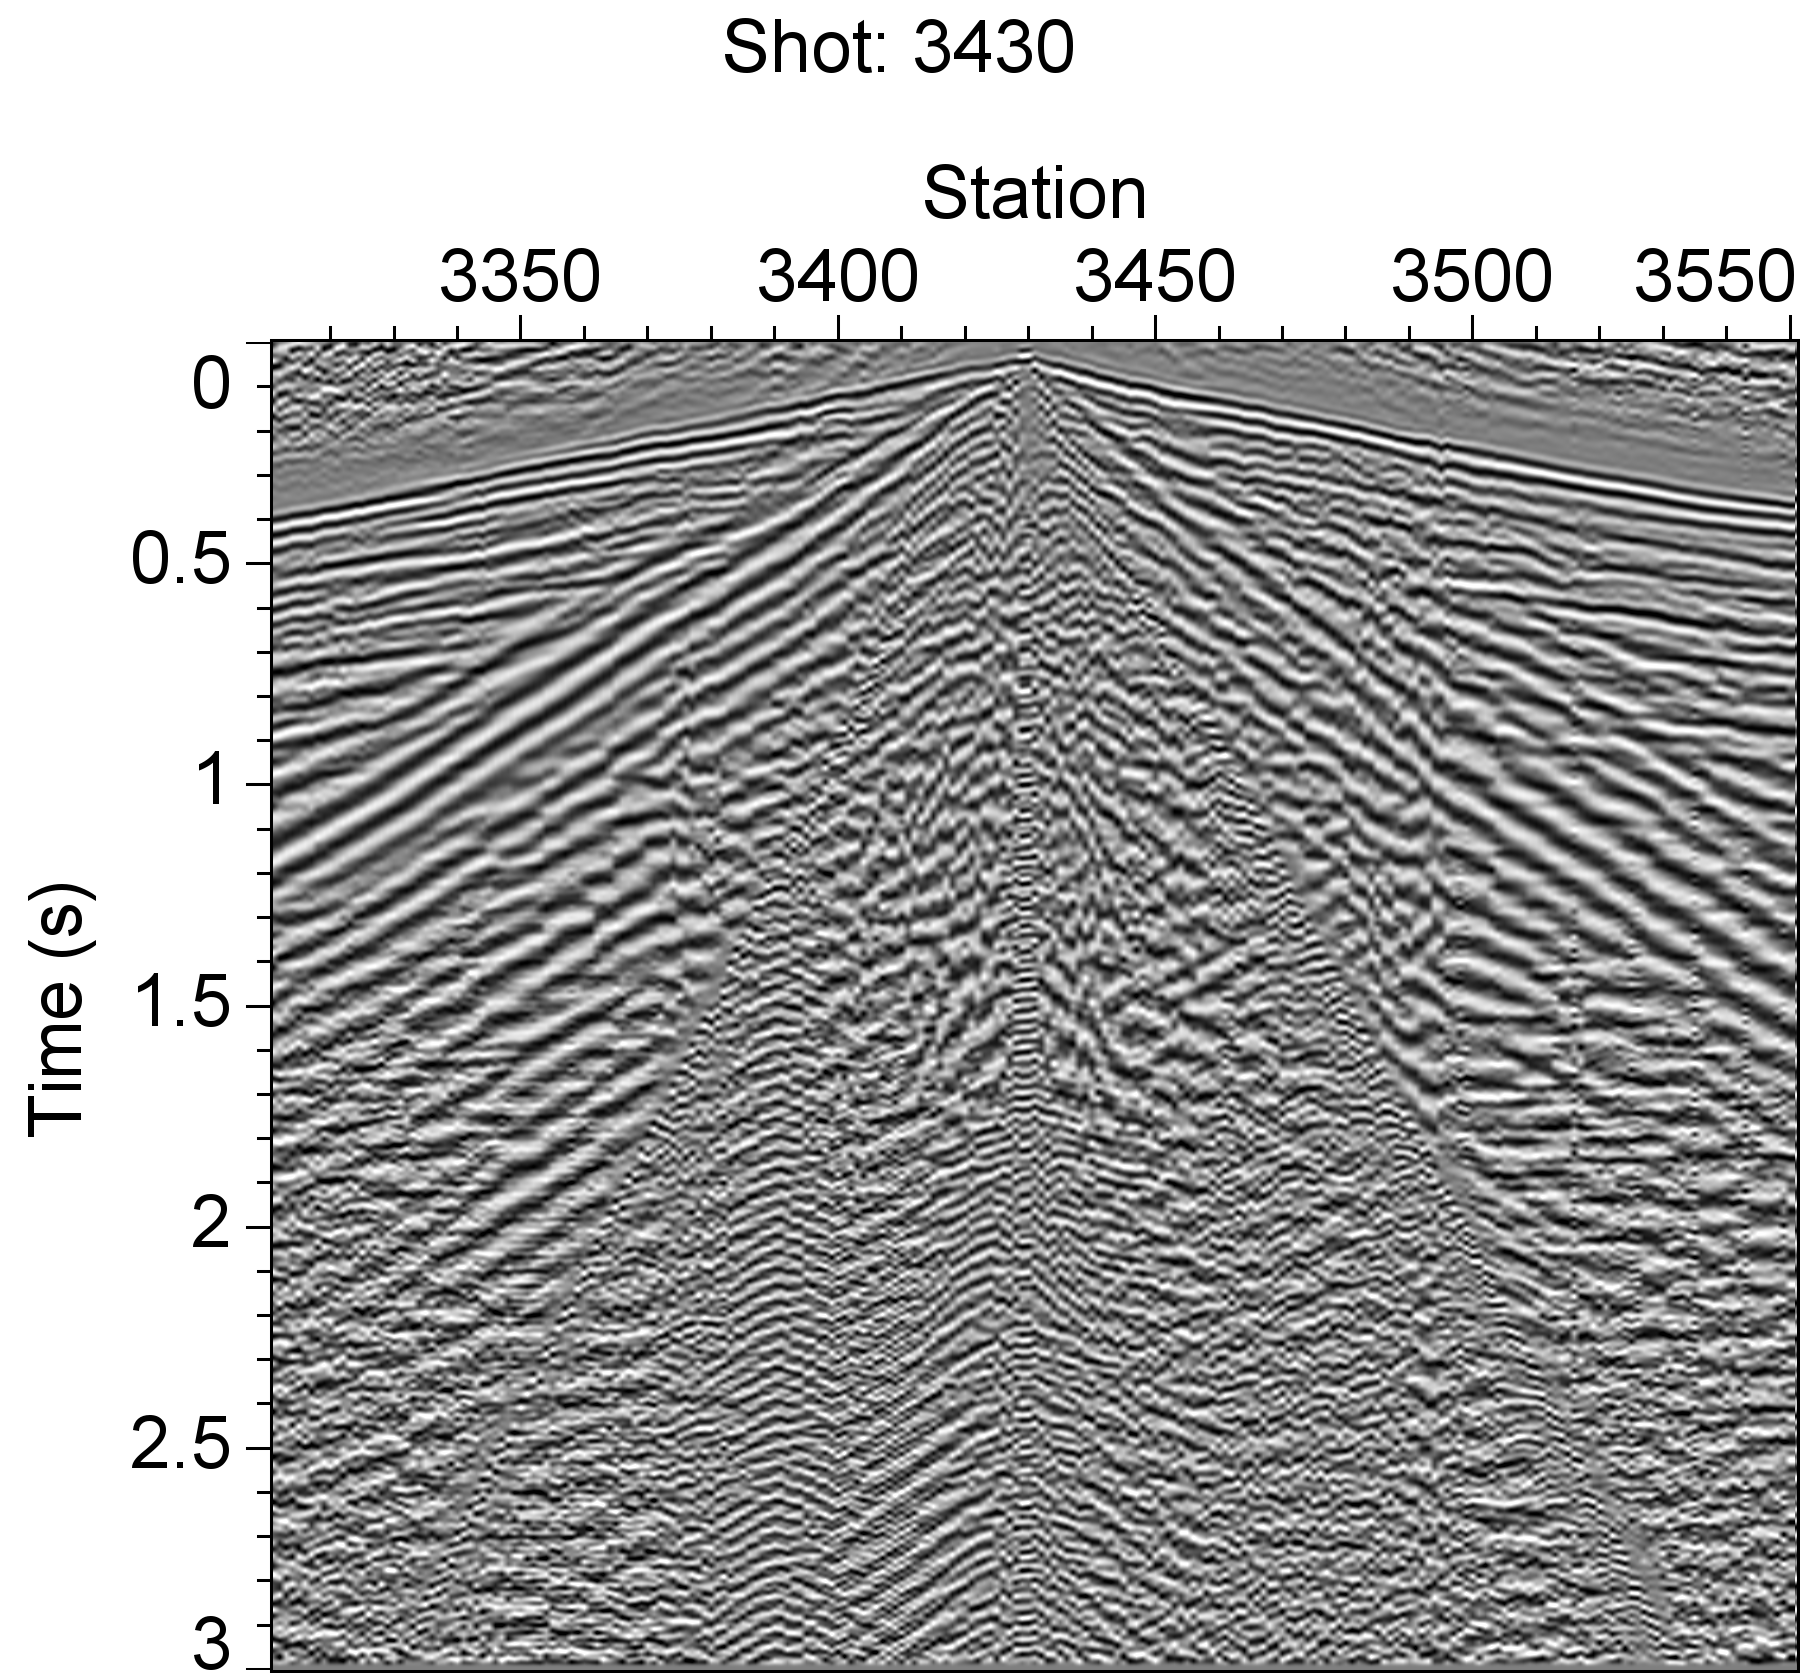
\includegraphics[width=0.75\textwidth]{./figs/fig4.png}
\caption{The Response Plot during Roam Mode with no summation. This shows a single shot record.}
\label{FIG:RP}
\end{figure}

\subsubsection{Roam Mode}

The Response Plot in Roam Mode will dynamically update based on the user's actions on the Base Plot. The shot points that are selected on the Base Map will be plotted on the Response Plot. If one shot is selected, then a shot record is displayed. If more shots are selected, a stack of those shots is displayed. Whenever the list of selected shots changes, the Response Plot will update with the new selection in this mode.

\begin{figure}[h]
\centering
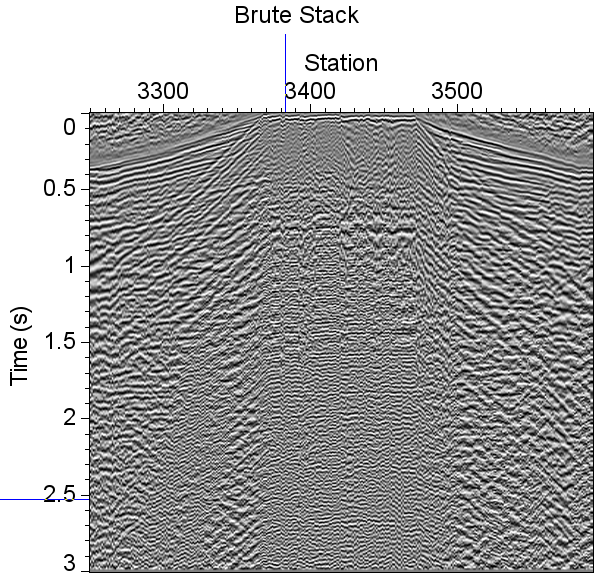
\includegraphics[width=0.75\textwidth]{./figs/fig3.png}
\caption{The Response Plot during Roam Mode showing an example stacked section.}
\label{FIG:RPR}
\end{figure}

\subsubsection{Circle Mode}

The Response Plot behaves the same way in Circle Mode as in Roam Mode. As the user expands the circle to select more shots on the Base Plot, a stack is created with the selected shot records. Every time the list of selected shots change, the Response Plot updates to the new set of data.

\subsubsection{Channel Mode}

In Channel Mode all the imported shots are automatically selected. In order to make a common channel section, the Response Plot has to update based off the Channel Slider. As the Channel Slider updates, the Response Plot creates common channel section based off of all the imported SEGD data. If there is no data at a particular shot, the Response Plot displays a vertical line for that station. A sample image of what to expect with a Common Channel Section would look like in the Response Plot is seen in Figure \ref{FIG:RPC}.

\begin{figure}[h]
\centering
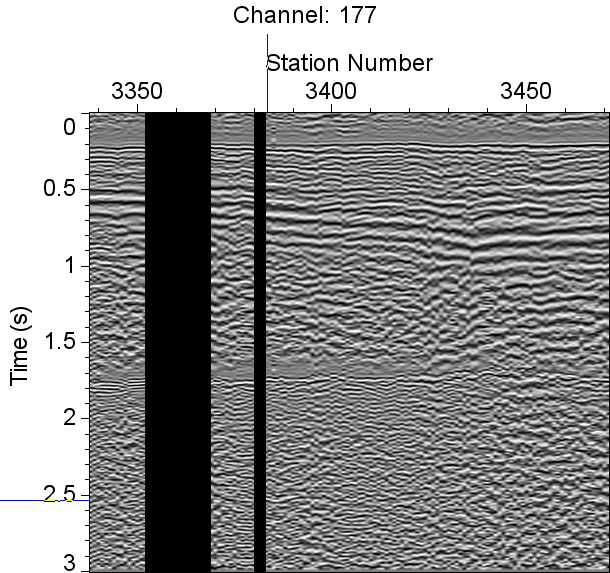
\includegraphics[width=0.75\textwidth]{./figs/fig5.png}
\caption{The Response Plot displaying a common channel section in Channel Mode.}
\label{FIG:RPC}
\end{figure}

\subsection{Secondary Controller - ElevPlot Class}
\label{SUBSEC:EP}

The Elevation Plot is controlled by the ElevPlot Class. When the GPS is first imported, the Elevation Plot updates with zero values. Then when the GPS elevations are updated from the NED files, the Elevation Plot updates with the true elevation values. Figure \ref{FIG:EP} shows what the Elevation Plot looks like after the GPS and the NED files have been imported and the NED files read.

\begin{figure}[h]
\centering
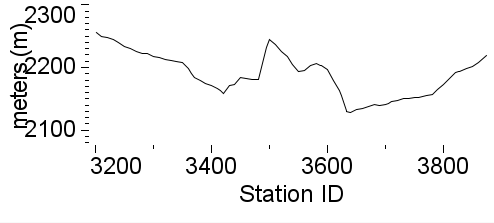
\includegraphics[width=0.75\textwidth]{figs/fig2.png}
\caption{Sample of the Elevation Plot profile after the NED files have been imported and read.}
\label{FIG:EP}
\end{figure}

\subsection{GPS Module - MPoint \& Waypoints Classes}

The MPoint and the Waypoints classes handles GPS points. An MPoint is essentially a map point with private fields for location in UTM and Latitude/Longitude coordinates. The MPoint class also includes methods for determining the distance between two MPoints. This is useful when trying to determine if an MPoint lies within a range of another MPoint (such as in Circle Mode). \\

Waypoints include methods for dealing with collections of MPoint objects. The methods in Waypoints includes tools for importing and exporting MPoint collections from and to files respectfully. Waypoints also has methods for determining the minimum and maximum station number. The Waypoints class can convert a list of MPoints' Latitude/Longitude into UTM Eastings and Northings. 

\subsection{NED Module - NedFile, NedFileHeader \& NedFileReader Classes}

The NedFile, NedFileHeader, and NedFileReader Classes are used for importing and reading NED files. The NedFile is composed of information about the north and west limits of the GridFloat file (extension ".flt"). \\

The NedFileHeader is where the information about the actual NedFile data is read and stored; that is, information such as the GridFloat file's cell size, lower left corner, and erroneous values. This all comes from the header file of the GridFloat file (extension ".hdr"). \\

The NedFileReader class contains methods for reading the NED GridFloat file and extracting an elevation given a Latitude and a Longitude. 

\subsection{SEGD Module - Segdata \& Segd Classes}

The final helper module has tools for reading and storing data that is pulled from SEGD files (extension ".segd"). The Segdata class is used to store the information about a particular shot. The important information includes the shot number (which is the same the GPS point), the line number, the beginning receiver station, the ending receiver station and the 2D float array of the shot data. \\ 

The Segd class includes tools for manipulating a list of Segdata objects including tools for importing the Segd files. It assumes that all SEGD files are in the Servel format and all files in a directory have the ".segd" extension. Segd also includes tools for applying gain, amplitude balance, and lowpass filters to the data. 

\section{Discussion and Conclusions}

This project developed software in Java that aids with the exploration of seismic data in the field. The program that was developed includes the interactive display of seismic survey geometry and shot records. This software is also able to perform simple processing tasks such as gain, amplitude correction, and lowpass filtering in the field. The program can also calculate and display brute stacks over a range of shots.  \\ 

While the program is far from an industry level program, it is a great start to a helpful field program. The documentation will aid future development and help the students at Field Camp explore the seismic data.

\section{Recommendations for Future Work}

The recommendations for future work fall into the categories of code cleanup and feature addition. The code cleanup will help with efficiency, speed and further development. Feature additions will help make the software more useful in the field. 

\subsection{Code Reorganization}

\begin{itemize}
\item More separation of the SeisPlot class and its internal classes. Currently, the SeisPlot class is composed of multiple inner. This can cause confusion when developing because it may not be clear to the programmer what parts of the code control what parts of the plot. It's my suggestion to separate the Plot classes from inside the SeisPlot class. From here, the SeisPlot class can function more as Main Controller with absolute control over everything and less of a Controller with shared power with its inner classes. A more modular design would also aid in development and allow for new features to be added with less code.

\item Optimization of search features. Currently the search algorithms used to find specific shots and map points is linear through an ArrayList. In order to maximize efficiency, a Binary Search Tree (BST) or Hash Map should be used for data storage.

\item Currently, the seismic survey's sampling rate is a constant 0.002 s/sample. This can easily change depending on the survey parameters. There needs to be a way to change this value in the program so the plots and processing can be useful in other survey parameters.
\end{itemize}

\subsection{Feature Addition}

\begin{itemize}

\item Reading and processing of observation reports. There is a whole set of data that has not been utilized for this program. The inclusion of this data could tell the user which channels are active and how much offset the shots have from the GPS station.

\item Expand the SEGD data import tool to include non-Sercel seismic data. This would require diving into different acquisition company's method of storing seismic data and programming logic to detect the type. A possible resource for this would be the Seismic Unix source code.

\item The ability to view ResponsePlot without GPS with a slider for shot number. In some cases, the GPS data might be acquired after the seismic data starts shooting. It would be helpful to still be able to view the seismic data by using a slider to display certain shot numbers. The current system is too dependent on GPS data for this type of robust viewing.

\item Extra tools for processing (kill ground roll, NMO correction, etc.). The python code provided by the client has several methods that are able to accomplish more processing that what is currently implemented. The reason these were not implemented in the current working version of the software was due to time constraints.

\item GPS needs more robust import/export system. The current regime only allows for very specific GPS formats to be imported. In order to be more robust, the user should be able to define the structure of the GPS data they want to import. The same should be true for exporting GPS data.

\item A UTM to Lat/Lon conversion. Currently the only supported mode for displaying GPS data is when it is in UTM coordinates. However, the only way to read the NED files is if the GPS data has Lat/Lon components. This could potentially cause a major issue if the GPS data is not read in as Lat/Lon data. 

\item A "save state" button. It would be helpful if the when the user closed down the program they could easily relaunch the program in the state they left it in. This may not be easily feasible because of the size of seismic surveys and the data storage requirements. One possibility for this would be to save the locations of the current imported data to a file and have those locations be re-imported.

\item The Elevation Plot should be more integrated into the activities on the base map. The Elevation Plot should have similar features as the Base Plot. Active shots should be coded with blue circles, active receivers with green crosses and the range of shots with a red line. As the user moves in Roam or Circle Mode along the Base Plot, the Elevation Plot should also update with selected shots.

\item The ability to export the imported SEGD files to the standard SEGY format would be helpful for post-field processing. The ability to import SEGY files could also be a large benefit to the end user.
\end{itemize}

\newpage
\section{References}

\printbibliography

\newpage
\section{Team Resume}

\begin{figure}[H]

\includegraphics[scale=0.80]{./Resume_of_Colton_Kohnke.pdf}
\end{figure}

\newpage
\section{Appendices}

\subsection{Java Program and Documentation}
The source code and documentation is available online at \url{https://github.com/voltnor/gp438/tree/master/novice}. The GPS data is included inside this github project. The 2013 Geophysics Field Camp seismic data and NED data is not stored online due to online file size limitations. 

\end{document}